\documentclass[a4paper, 10pt]{article}
\usepackage{fullpage}
\usepackage{titling}
\usepackage{graphics}
\usepackage{amsmath}
\usepackage{amssymb}
\usepackage{hyperref}
\usepackage{IEEEtrantools}
\usepackage{graphicx}
\usepackage{tcolorbox}
\usepackage{xcolor}
\usepackage[normalem]{ulem}

\setlength{\droptitle}{-6em}   % This is your set screw, for shifting up the title
\renewcommand{\baselinestretch}{1.1}
\setlength{\parskip}{0.5em}

\author{}
\date{}
\title{Worksheet 7 \vspace{-0.5cm}}

\DeclareMathOperator{\E}{\mathbb{E}}
\DeclareMathOperator{\V}{\mathbb{V}}

\begin{document}
\maketitle
\vspace{-2cm}

\subsubsection*{Q1}
(\textit{Exercise 6.1 S\&B})
If $V$ changes during the episode, then
$$G_{t} - V(S_{t}) = \sum_{k=t}^{T-1}\gamma^{{k-1}}\delta_{k} $$
only holds approximately; what would the difference be between the two sides? Let $V_{t}$ denote the array of state values used at time $t$ in the TD error and in the TD update.
Redo the derivation to determine the additional amount that must be added to the sum of TD errors in order to equal the Monte Carlo error.

\subsubsection*{Answer:}
With the given notation, $\delta_t = R_{t+1} + \gamma V_t(S_{t+1}) - V_t(S_t)$. The required derivation is as follows:
\begin{IEEEeqnarray*}{lCl}
  G_t - V_t(S_t) &=& R_{t+1} + \gamma G_{t+1} - V_t(S_t) + \gamma V_t(S_{t+1}) - \gamma V_t(S_{t+1}) \\
  &=& \delta_t + \gamma (G_{t+1} - V_t(S_{t+1})) \\
  &=& \delta_t + \gamma (G_{t+1} - V_{t+1}(S_{t+1})) + \gamma (V_{t+1}(S_{t+1}) - V_t(S_{t+1})) \\
  &=& \delta_t + \gamma \big[\delta_{t+1} + \gamma (G_{t+2} - V_{t+2}(S_{t+2})) + \gamma (V_{t+2}(S_{t+2}) - V_{t+1}(S_{t+2})) \big] + \gamma (V_{t+1}(S_{t+1}) - V_t(S_{t+1})) \\
  &=& \delta_t + \gamma \delta_{t+1} + \gamma^2 (G_{t+2} - V_{t+2}(S_{t+2})) + \gamma^2 (V_{t+2}(S_{t+2}) - V_{t+1}(S_{t+2})) + \gamma (V_{t+1}(S_{t+1}) - V_t(S_{t+1})) \\
  &\vdots& \\
  &=& \delta_t + \gamma \delta_{t+1} + \cdots + \gamma^{T-t-1} \delta_{T-1} + \gamma^{T-t} (G_t - V_T(S_T)) \\
  && \quad \quad + \gamma^{T-t} (V_T(S_T) - V_{T-1}(S_T)) + \cdots + \gamma (V_{t+1}(S_{t+1}) - V_t(S_{t+1})) \\
  &=& \sum_{k=t}^{T-1} \gamma^{k-t} \delta_k + \gamma \sum_{k=t}^{T-1} \gamma^{k-t} (V_{k+1}(S_{k+1}) - V_k(S_{k+1})).
\end{IEEEeqnarray*}

If the learning rate is small, then $V_{k+1}(S_{k+1}) \approx V_k(S_{k+1})$, and the equality given in the question would hold.

\subsubsection*{Q2}
(\textit{Exercise 6.3 S\&B})
From the results shown in the left graph of the random walk example it
appears that the first episode results in a change in only $V(A)$.
What does this tell you about what happened on the first episode?
Why was only the estimate for this one state changed?
By exactly how much was it changed?
\begin{figure}[h!]
\centering
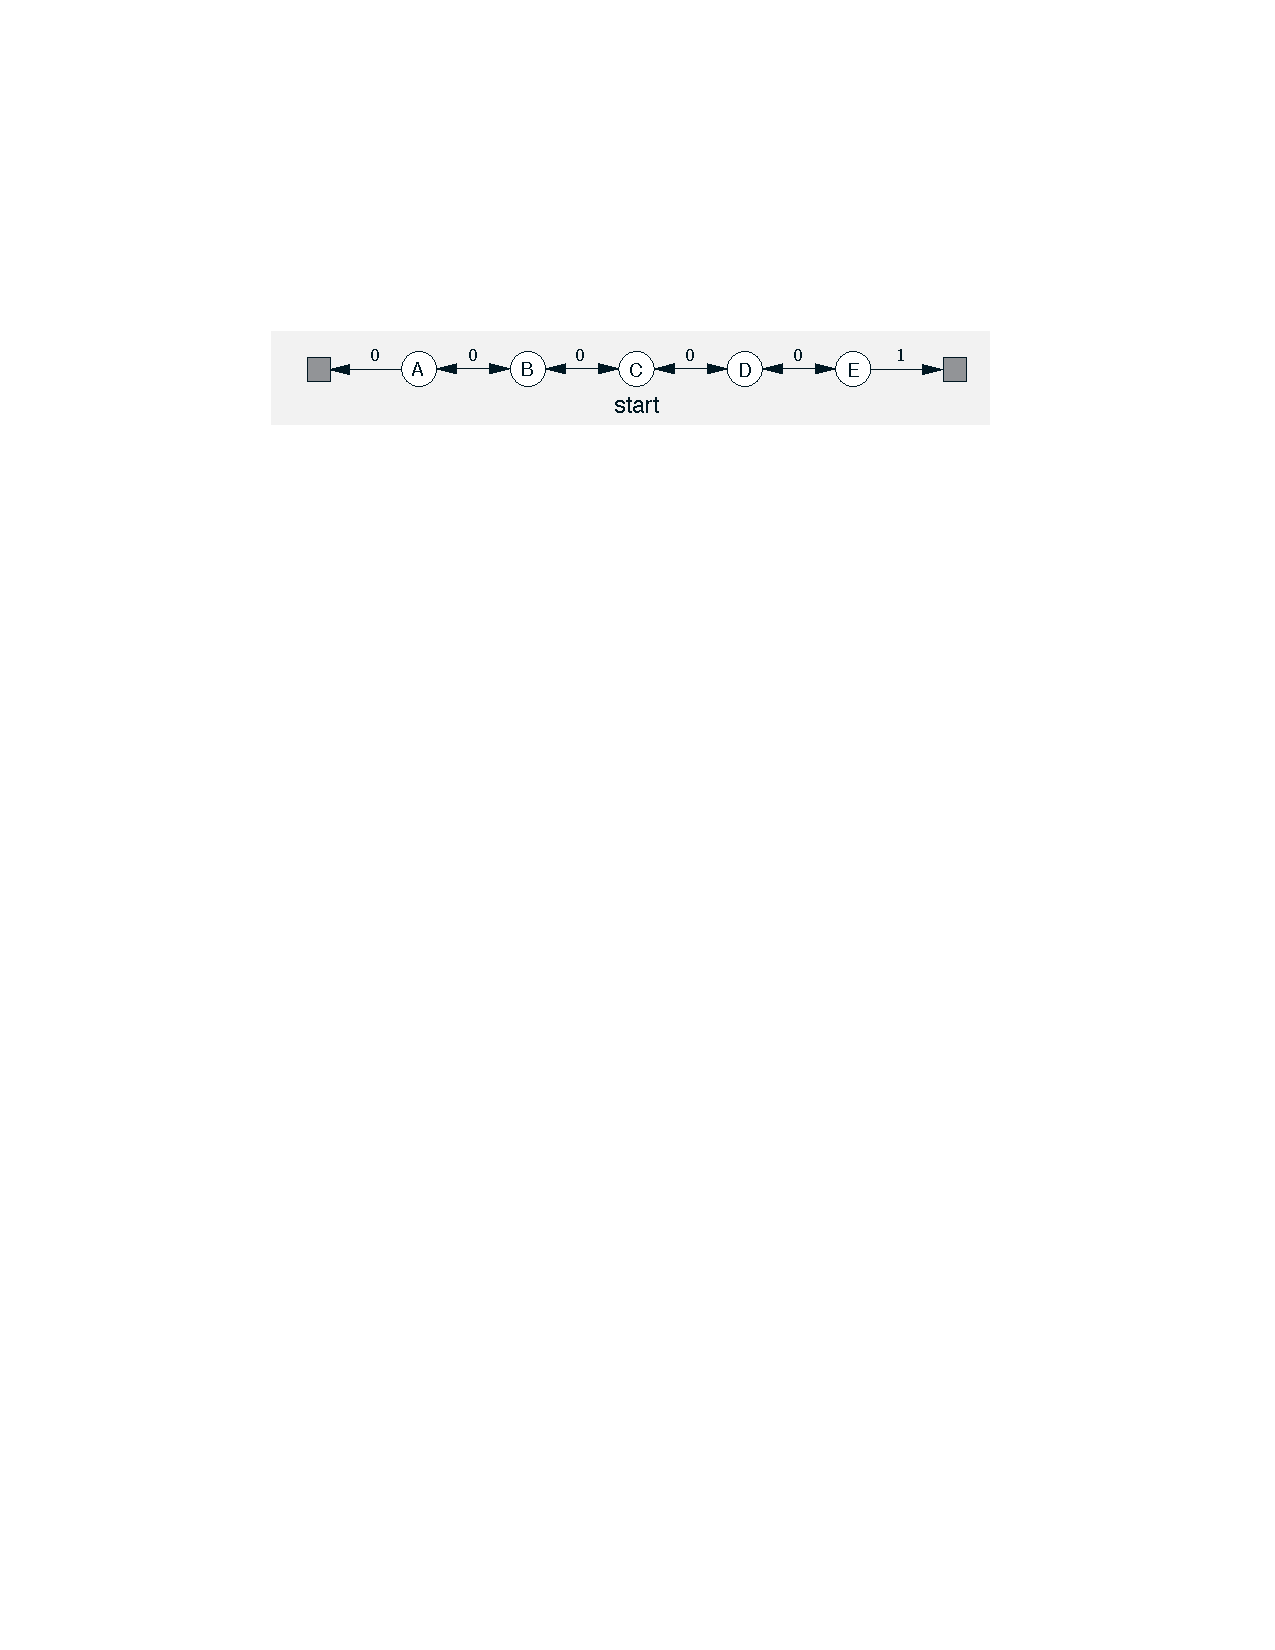
\includegraphics[scale=0.9]{figures/c2m2_rw.pdf}
\end{figure}
\begin{figure}[h!]
\centering
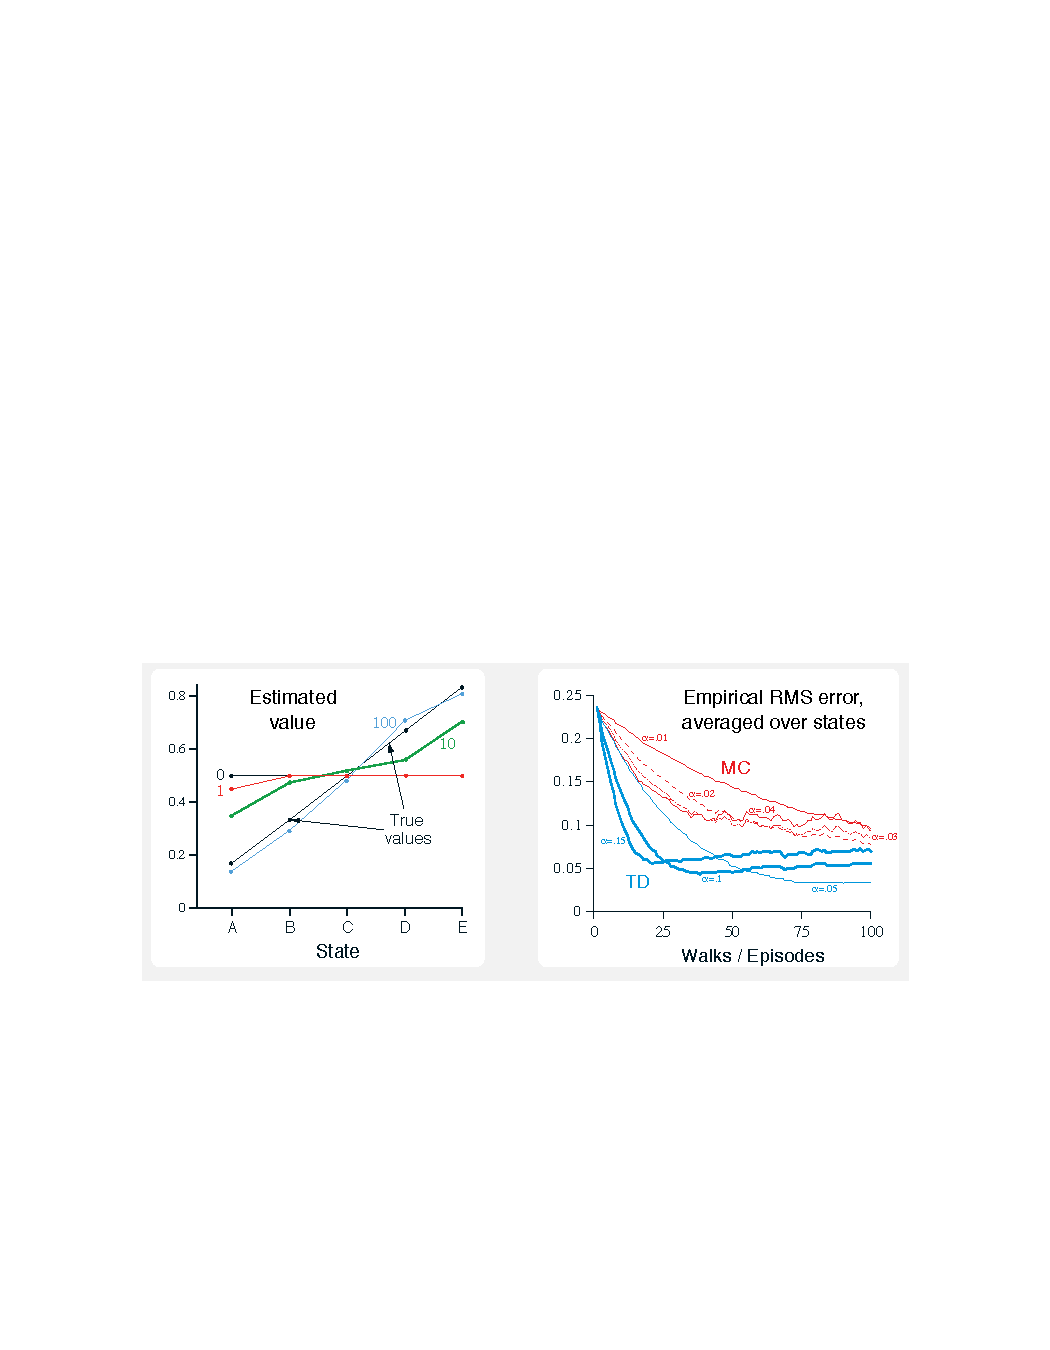
\includegraphics[scale=0.9]{figures/figure_6dot2.pdf}
\end{figure}

\subsubsection*{Answer:}
The initial estimate $V(A) = 0.5$. Since, the estimate decreases, the episode must have ended in the left terminal state. Let us denote the left terminal state by $L$. Then the last transition of the episode is: $(S=A, R=0, S'=L)$. The update corresponding to this transition is:
\begin{IEEEeqnarray*}{lCl}
  V(A) &=& V(A) + 0.1 [0 + V(L) - V(A)] \\
  &=& 0.5 + 0.1 [0 + 0 - 0.5] \\
  &=& 0.45.
\end{IEEEeqnarray*}

For all other transitions $(S, R=0, S')$ with $S' \notin \{L, R\}$ with $R$ denoting the right terminal state, the updates would be: $V(S) = V(S) + 0.1 [0 + V(S') - V(S)] = V(S)$, since at the beginning of the episode $V(S) = V(S') = 0.5$.

\subsubsection*{Q3}
(\textit{Exercise 6.4 S\&B})
The specific results shown in the right graph of the random walk example are dependent on the value of the step-size parameter, $\alpha$.
Do you think the conclusions about which algorithm is better would be affected if a wider range of $\alpha$ values were used?
Is there a different, fixed value of $\alpha$ at which either algorithm would have performed significantly better than shown? Why or why not?

\subsubsection*{Answer:}
Most likely the conclusion that TD is better than Monte Carlo on this method won't change with a wider range of stepsizes. For the MC curve, we can see that the final performance of MC method is best at an intermediate value of $\alpha=0.03$. This is characteristic of performance against parameters (parameter studies) --- an intermediate value of parameters performs better than extreme values. As a result, trying higher and smaller values of $\alpha$ won't likely bring a big difference in the final performance of the MC method. And since the best performance of MC for $\alpha=0.03$ is still worse than the worst TD, the conclusions should remain the same that TD is superior to MC in this setting. Similarly, for TD, tuning the stepsize wouldn't create a big difference in terms of performance. \textcolor{red}{For TD this answer is vague. Maybe add a discussion about TD bounds}.

\subsubsection*{Q4}
\textbf{(Challenge Question)} (\textit{Exercise 6.5 S\&B}) In the right graph of the random walk example, the RMS error of the
TD method seems to go down and then up again, particularly at high $\alpha$'s.
What could have caused this?
Do you think this always occurs, or might it be a function of how the approximate value function was initialized?

\subsubsection*{Answer:}
\textcolor{red}{This is based on Rupam's PhD thesis (Section 9.7). I don't understand this very well and I'm unable to explain this in a simple and intuitive manner.} These forms of oscillations are charecteristic for TD algorithm, since the matrix ${\bf A}$ in the TD update equations is assymetric and as a result, the imaginary parts of its eigenvalues are non--zero. This causes the oscillations seen in the figure. \textcolor{red}{I don't think it would depend on how the value function was initialized}.


\subsubsection*{Q5}
(\textit{Exercise 6.7 S\&B}) Design an off-policy version of the TD(0) update that can be used with arbitrary target policy $\pi$ and covering behavior policy $b$, using at each step $t$ the importance sampling ratio $\rho_{t:t}$ (5.3).

\subsubsection*{Answer:}
In this question, we only update the target $(R + \gamma V(S'))$ of the TD--update. We'll ignore the stationary state distribution. This setting is also called the excursion setting. We begin by writing the Bellman equation and then modifying it to obtain the off--policy TD update.
\begin{IEEEeqnarray*}{lCl}
  V_\pi(s) &=& \sum_a \pi(a|s) \sum_{s', r} p(s', r|s, a) [r + \gamma V_\pi(s')] \\
  &\equiv& \E_{\pi, P} [R_{t+1} + \gamma V(S_{t+1}) | S_t = s] \\
  &=& \sum_a b(a|s) \underbrace{\frac{\pi(a|s)}{b(a|s)}}_{\rho_{t:t}} \sum_{s', r} p(s', r|s, a) [r + \gamma V_\pi(s')] \\
  &\equiv& \E_{b, P} [\rho_{t:t} (R_{t+1} + \gamma V(S_{t+1})) | S_t = s].
\end{IEEEeqnarray*}

The last line leads to the following off--policy TD update:
\begin{equation} \label{eq: td_one}
  V(S_t) = V(S_t) + \alpha [\rho_{t:t} (R_{t+1} + \gamma V(S_{t+1})) - V(S_t)].
\end{equation}

There is an alternate algorithm as well. We write $\E_{\pi, P} [\delta_t | S_t = s] \equiv \E_{\pi, P} [R_{t+1} + \gamma V(S_{t+1}) - V(S_t)] = \E_{\pi, P} [\rho_{t:t} \delta_t | S_t = s]$. This leads to the following alternate TD algorithm:
\begin{equation} \label{eq: td_two}
  V(S_t) = V(S_t) + \alpha \rho_{t:t} [R_{t+1} + \gamma V(S_{t+1}) - V(S_t)].
\end{equation}

Note that the expected update, under the behavior policy, in both Eq. \ref{eq: td_one} and \ref{eq: td_two} is same:
\begin{equation*}
  \E_{b, P} [\rho_{t:t} (R_{t+1} + \gamma V(S_{t+1})) - V(S_t) | S_t] = \E_{b, P} [\rho_{t:t}(R_{t+1} + \gamma V(S_{t+1}) - V(S_t)) | S_t].
\end{equation*}
It is straightforward to see this by using the linearity of the expectation operator and the fact that $\E_{b, p}[\rho_t | S_t] = \sum_a b(a|s) \frac{\pi(a|s)}{b(a|s)} = 1$.

\subsubsection*{Q6}
Modify the Tabular TD(0) algorithm for estimating $v_\pi$, to estimate $q_\pi$.
\begin{figure}[h!]
  \center
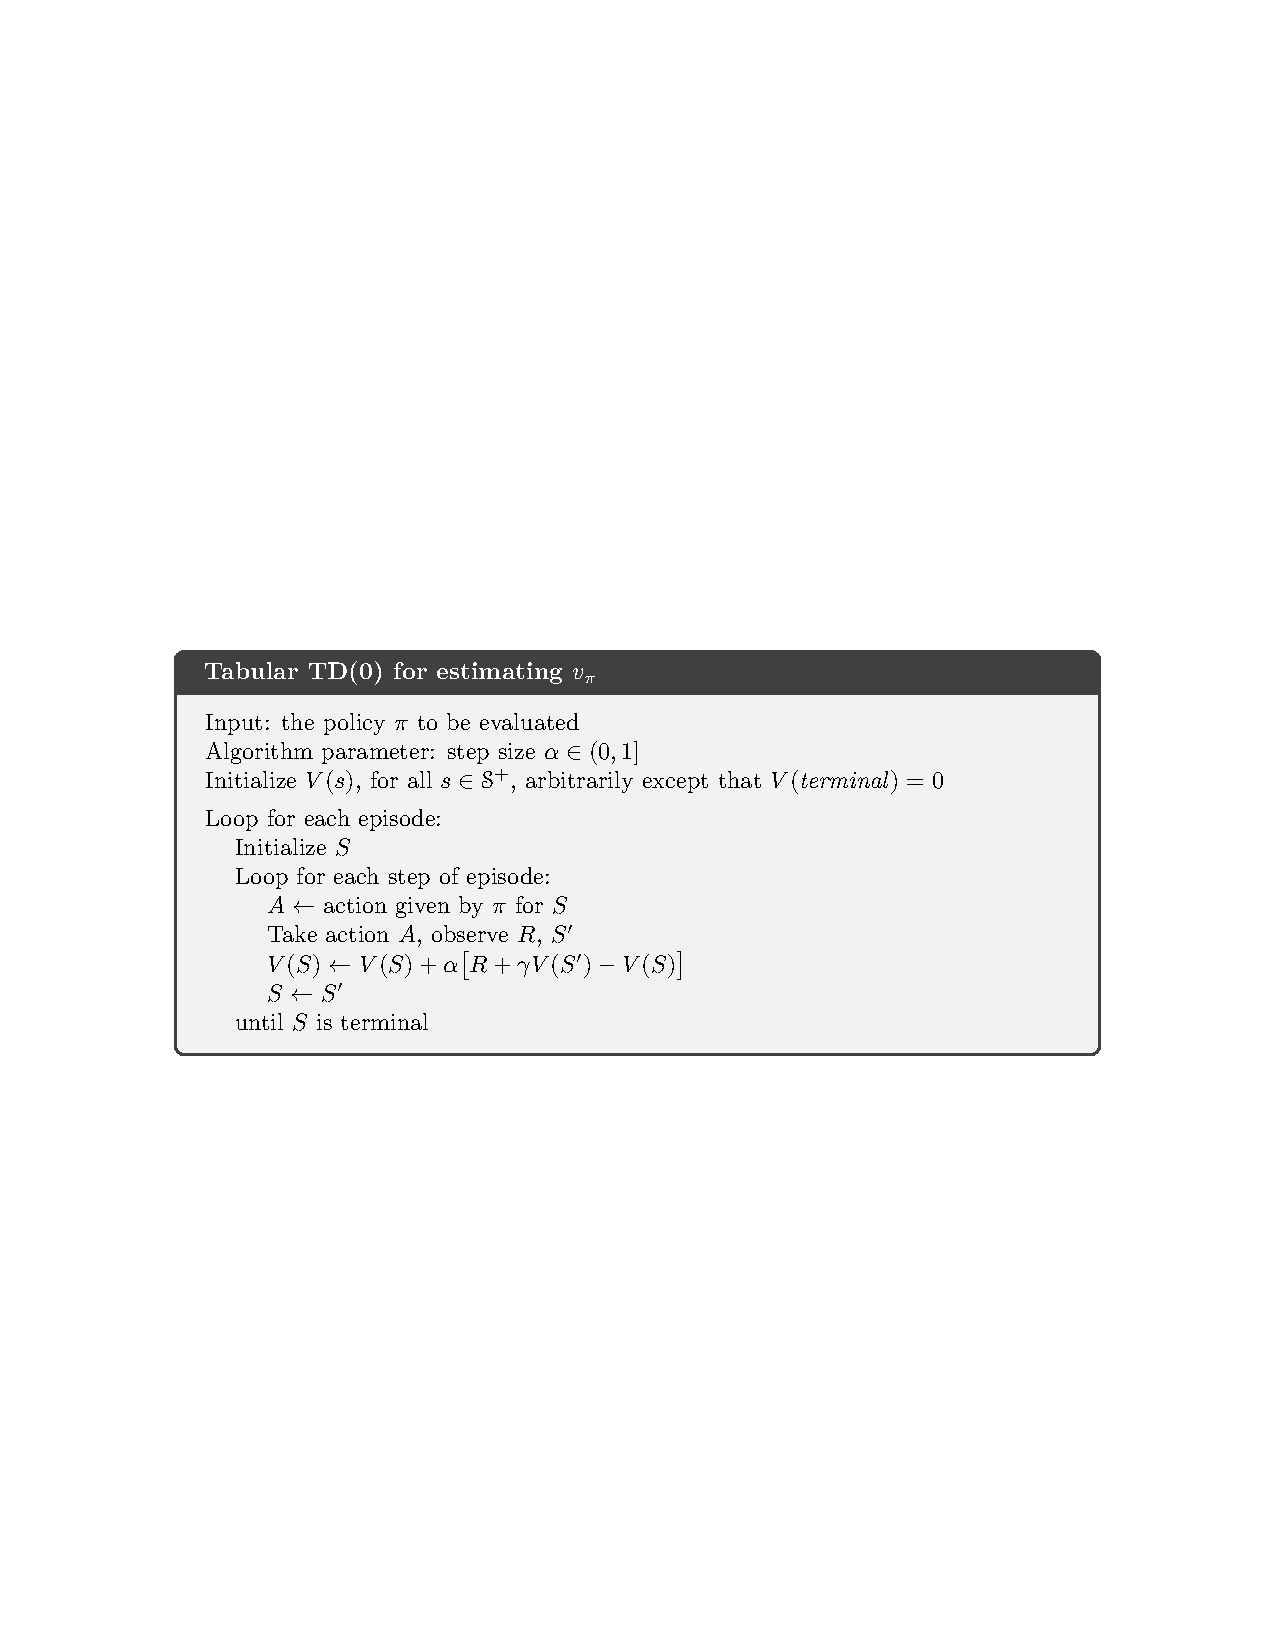
\includegraphics[width=0.85\linewidth]{figures/c2m2_td_alg.pdf}
\end{figure}

\subsubsection*{Answer:}
\begin{tcolorbox}[title=Tabular TD(0) for estimating $q_\pi$]
  Input: the policy $\pi$ to be evaluated \\
  Algorithm parameter: step size $\alpha \in (0, 1]$ \\
    Initialize $Q(s, a)$, for all $s \in \mathcal{S}^+$, $a \in \mathcal{A}(s)$, arbitrarily except that $Q(terminal, \cdot) = 0$ \\ \\
    Loop for each episode: \\
    \phantom{---} Initialize $S$ \\
    \phantom{---} Choose action $A$ given by $\pi$ for $S$ \\
    \phantom{---} Loop for each step of episode \\ 
    \phantom{---} \phantom{---} Take action $A$, observe $R, S'$ \\
    \phantom{---} \phantom{---} Choose action $A'$ given by $\pi$ for $S'$ \\
    \phantom{---} \phantom{---} $Q(S, A) \leftarrow Q(S, A) + \alpha [R + \gamma Q(S', A') - Q(S, A)]$ \\ 
    \phantom{---} \phantom{---} $S \leftarrow S'; A \leftarrow A';$ \\
    \phantom{---} until $S$ is terminal. 
\end{tcolorbox}

\subsubsection*{Q7}
Suppose that in an environment, state transitions are deterministic and that reward is bounded so that $R_{min} = 0$ and $R_{max} = 1$, with $\mathbb{E}[R_{t}] = 0.5$. Find the maximum and minimum possible TD error $\delta_{t} = R_{t+1} + \gamma V(S_{t+1}) - V(S_{t})$, where $\gamma = 0.9$ and $V = v_{\pi}$ with deterministic policy $\pi$.
% max: 1 - 0.5 = 0.5
% min: 0 - 0.5 = -0.5

\subsubsection*{Answer:}
We know that the for the exact value function $v_\pi$,
\begin{equation*}
  v_\pi(S_t) = \E[R_{t+1} + \gamma v_\pi(S_{t+1})] = \E[R_{t+1}] + \gamma v_\pi(S_{t+1}).
\end{equation*}
Therefore, we can write
\begin{IEEEeqnarray*}{lCl}
  \delta_t &=& R_{t+1} + \gamma v_\pi(S_{t+1}) - v_\pi(S_t) \\
  &=& R_{t+1} + \gamma v_\pi(S_{t+1}) - \E[R_{t+1}] - \gamma v_\pi(S_{t+1}) \\
  &=& R_{t+1} - \E[R_{t+1}] \\
  &=& R_{t+1} - 0.5.
\end{IEEEeqnarray*}

Therefore, the maximum TD error is $\delta = R_{\text{max}} - 0.5 = 0.5$ and the minimum TD error is $\delta = R_{\text{min}} - 0.5 = -0.5$.

\subsubsection*{Q8}
Assume the agent interacts with a simple two-state MDP shown below. Every episode begins in state $X$, and ends when the agent transitions from state $Y$ to the terminal state (denoted by gray box). Let's denote the set of states as $\mathcal{S} = \{X,Y,T\}$. There is only one possible action in each state, so there is only one possible policy in this MDP. Let's denote the set of actions $\mathcal{A} = \{A\}$. In state $Y$ the agent terminates when it takes action $A$ and sometimes gets a reward of +1000, and sometimes gets a reward of -1000: the reward on this last transition is stochastic. Let $\gamma = 1.0$. 
\begin{figure}[h!]
  \center
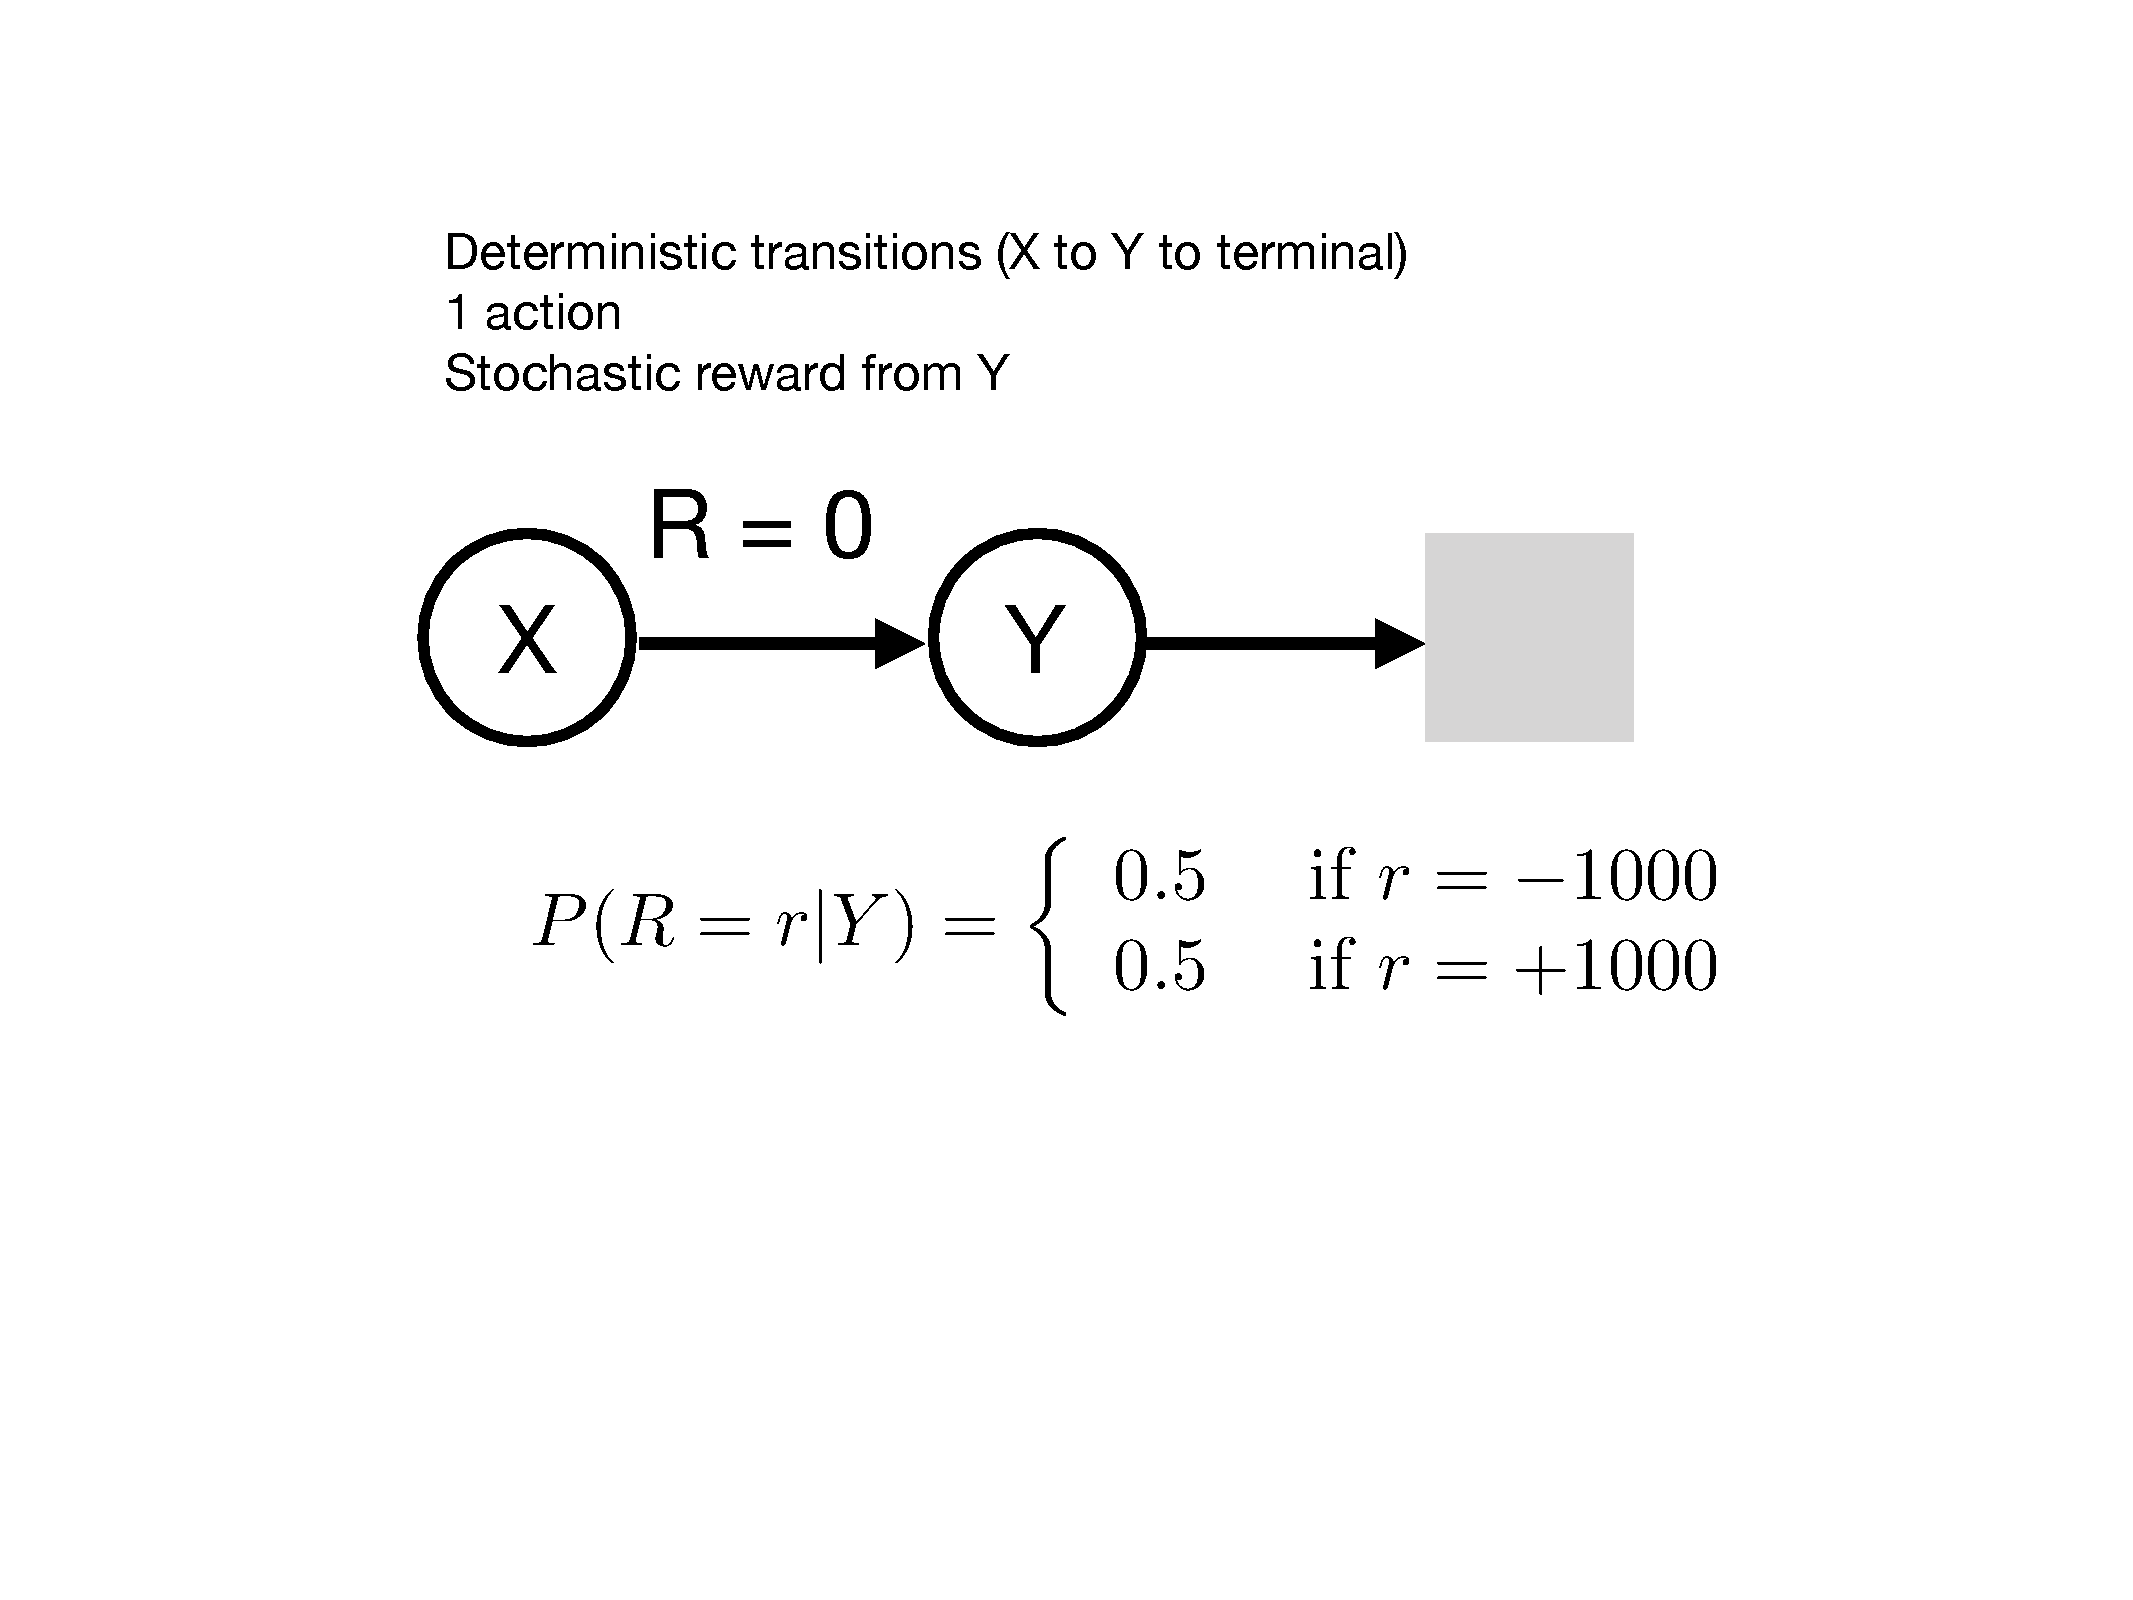
\includegraphics[width=0.5\linewidth]{figures/c2m2_xy.pdf}
\end{figure}
%
\begin{enumerate}
%
\item Write down $\pi(a|s) ~\forall~ s\in\mathcal{S}, a\in\mathcal{A}$
\item Write down all the possible trajectories (sequence of states, actions, and rewards) in this MDP that start from state $X$?
\item What the value of policy $\pi$ (i.e. what is $v_\pi(X), v_\pi(Y)$)?
\item Assume our estimate is equal to the value of $\pi$. That is $V(s) = v_\pi(s) ~\forall~ s\in\mathcal{S}$. Now compute the TD-error $\delta_t = R_{t+1} + \gamma V(S_{t+1}) - V(S_t)$ for the transition from state $Y$ to the terminal state, assuming $R_{t+1} = +1000$. Why is the TD-error not zero if we start with $V(Y) = v_\pi(Y)$?
\item Based on your answer to (e), what does this mean for the TD-update, for constant $\alpha = 0.1$? Will $V(Y) = v_\pi(Y) = 0$ after we update the value? Recall the TD-update is $V(S_t) \gets V(S_t) + \alpha \delta_t$.  What does this tell us about the updates TD(0) would make on this MDP?
\item What is the expected TD-update, from state $Y$ for the given $V$?
\item Assume still that $V=V_\pi = 0$. What is the expectation and the variance of the TD update from state $X$? What is the expectation and the variance of the Monte-carlo update from state $X$?
\end{enumerate}

\subsubsection*{Answer:}
\begin{enumerate}
\item $\pi(A|X) = 1$ and $\pi(A|Y) = 1$.
\item $(S_0=X, A_0=A, R_1=0, S_1=Y, A_1=A, R_2=1000, S_2=T)$ and $(S_0=X, A_0=A, R_1=0, S_1=Y, A_1=A, R_2=-1000, S_2=T)$.
\item We know that $v_\pi(S) = \sum_a \pi(a|s) \sum_{s', r} p(s', r | s, a) [r + \gamma v_\pi(s')]$ and that $v_\pi(T) \doteq 0$. Using this $v_\pi(Y) = 1\cdot[0.5 (1000 + \gamma v_\pi(T)) + 0.5 (-1000 + \gamma v_\pi(T))] = 0$ and $v_\pi(X) = 1 \cdot 1 \cdot [0 + \gamma v_\pi(Y)] = 0$.
\item $\delta_t = R_{t+1} + \gamma v_\pi(S_{t+1}) - v_\pi(S_t) = 1000 + \gamma v_\pi(T) - v_\pi(Y) = 1000$. The TD error is zero in expectation for the true value function, i.e. $\E[\delta_t | S_t] = 0$ for $v_\pi$ as we later show. Its value doesn't have to be zero.
\item Based on the above sub--question, if we make the TD update for state $Y$ using $\alpha=0.1$, we would obtain: $V(Y) = V(Y) + 0.1 \times 1000 = 100$. If we continue to make such updates, we can see that $V(Y)$ will oscillate without ever going to zero.
\item $\E[\delta_t | S_t] = \sum_{r} p(r | Y) (r + \gamma v_\pi(T) - v_\pi(Y)) = 0.5 (1000 + \gamma v_\pi(T) - v_\pi(Y)) + 0.5 (-1000 + \gamma v_\pi(T) - v_\pi(Y)) = 0$.
\item
  \textbf{TD update:} \textcolor{red}{I'm not sure about this.} The expectation of the TD update is
   \begin{equation*}
    \E[\delta | X] = \E[0 + \gamma v_\pi(Y) - v_\pi(X) | X] = 0,
  \end{equation*}
   since each $v_\pi(X) =  v_\pi(Y)  = 0$.
   The variance of the TD update is
   \begin{IEEEeqnarray*}{lCl}
      \V[\delta | X] &=& \E[\delta^2 | X] - \E[\delta | X]^2\\
      &=& \E[(0 + \gamma v_\pi(Y) - v_\pi(X))^2 | X] \\
      &=& 0.
    \end{IEEEeqnarray*}
  \textbf{MC update:} The expectation of the MC update is
  \begin{equation*}
    \E[G - v_\pi(X) | X] = 0.5 \times1000 + 0.5 \times(-1000) = 0.
  \end{equation*}

  Similarly, the variance is
    \begin{IEEEeqnarray*}{lCl}
      \V[G - v_\pi(X) | X] &=& \E[(G - v_\pi(X))^2 | X] - \E[G - v_\pi(X) | X]^2\\
      &=& \E[(G - v_\pi(X))^2 | X] \\
      &=& 0.5 \times1000^2 + 0.5 \times(-1000)^2 \\
      &=& 1000^2.
    \end{IEEEeqnarray*}
\end{enumerate}

\subsubsection*{Q9}
(\textbf{Challenge Question})
In this question we consider the variance of the TD target, $R_{t+1} + \gamma V(S_{t+1})$ compared to the variance of the Monte Carlo target, $G_t$. Let's assume an idealized setting, where we have found a $V$ that exactly equals $v_\pi$. We can show that, in this case, the variance of the Monte Carlo target is greater than or equal to the variance of the TD target. Note that variance of the targets is a factor in learning speed, where lower variance targets typically allow for faster learning. Show that  the Monte Carlo target has at least as high of variance as the TD target, using the following decomposition, called the Law of Total Variance
%
\begin{align*}
\text{Var}(G_t) = \mathbb{E}[\text{Var}(G_t | S_{t+1})] + \text{Var}(\mathbb{E}[G_t | S_{t+1}])  
.
\end{align*} 
%
Note that the above means the variance of the return given state $S_t = s$: $\text{Var}(G_t | S_t = s)$. We omit the given $S_t = s$ from the above, to make it more readable, but implicitly it is there (i.e. the above equation is: $\text{Var}(G_t | S_t = s) = \mathbb{E}[\text{Var}(G_t | S_t = s, S_{t+1})] + \text{Var}(\mathbb{E}[G_t | S_t = s, S_{t+1}] | S_t = s)  $). Further, to better understand the double expectations, 
%
\begin{align*}
\mathbb{E}[G_t] = \mathbb{E}[\mathbb{E}[G_t | S_{t+1}]] = \sum _{s' \in \mathcal{S}} p(s' | S_t = s) \mathbb{E}[G_t | S_{t+1}]
.
\end{align*} 
%
The outer expectation is over $S_{t+1}$, with the inner expectation computed given $S_{t+1}$. Similarly, 
%
\begin{align*}
\mathbb{E}[\text{Var}(G_t | S_{t+1})]  = \text{\sout{$\mathbb{E}[\mathbb{E}[G_t | S_{t+1}]]$}} = \sum _{s' \in \mathcal{S}} p(s' | S_t = s) \text{Var}[G_t | S_{t+1}]
.
\end{align*} 
% 
To answer the above question, try to simplify $\text{Var}(\mathbb{E}[G_t | S_{t+1}])$ by showing that $\mathbb{E}[G_t | S_{t+1}] = R_{t+1} + \gamma V(S_{t+1})$. Notice that this is only true because $V(S_{t+1}) = v_\pi(S_{t+1})$.
Then conclude that this implies  
%
\begin{align*}
\text{Var}(G_t) \ge \text{Var}(R_{t+1} + \gamma V(S_{t+1}))  
.
\end{align*} 
%
%%
%\begin{align*}
%\text{Var}(G_t | S_t = s) = \mathbb{E}[\text{Var}(G_t | S_t = s, S_{t+1})] + \text{Var}(\mathbb{E}[G_t | S_t = s, S_{t+1}] | S_t = s)  
%.
%\end{align*} 
%%

\subsubsection*{Answer:}

\end{document}
